\documentclass[11pt, a4paper,twocolumn]{jarticle}
\usepackage[dvipdfmx]{graphicx}
\usepackage{listings,jlisting}

\begin{document}
%=============================================================
\section{Measurement of the temperature dependence of the resistivity of $Bi_2Sr_2Ca_2Cu_3O_{10}$ as a superconductor($6^{th} day$)}

\subsection{Purpose}
超電導の転移温度の測定を通して超電導の原理について学ぶ.
\subsection{Procedure}
前回同様に図\ref{fig:29}のように温度依存性の測定のための実験装置を組み立てる.
次に超電導リボン($Bi_2Sr_2Ca_2Cu_3O_{10}$)の電圧-電流特性を四端子測定法で測定する.
この時超電導のヒステリシス特性を観察するために室温から超電導が起こる相転移温度まで下げていった場合と,超電導状態から室温に近づけていった場合の二パターンについて測定を行いそれぞれの結果を温度-抵抗値のグラフにプロットしていく.
測定の際は電流が100mAを超えないように注意して行う.

\subsection{Result}
測定の結果温度と抵抗値の関係をプロットすると以下のようなグラフが得られた.
ヒステリシスが測定され,室温から温度を下げていった場合よりも超電導状態から室温にあげていった時は結果が全体的に左にシフトした.
また実験結果より温度下降時は相転移温度は140Kほど,上昇時は130Kほどであることが確認された.

\begin{figure}[htbp]
 \begin{center}
  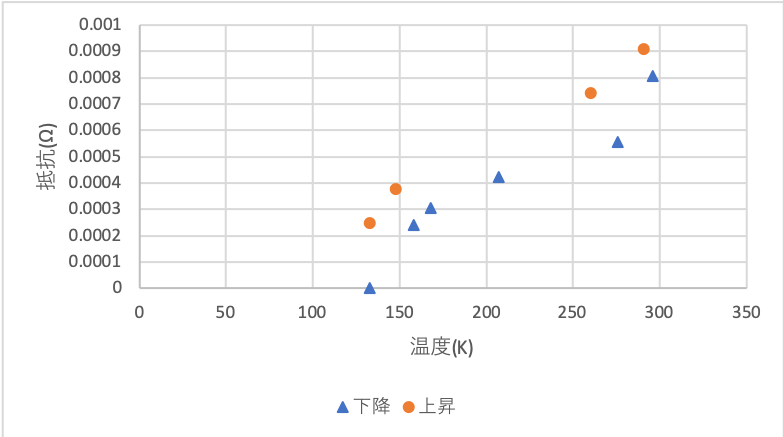
\includegraphics[width=0.8\linewidth]{fig39.png}
 \end{center}
 \caption{温度下降}
 \label{fig:39}
\end{figure}

\subsection{Discussion}
超電導が起こる理由について考える.
まず超電導が起きる極低温状態においては原子の熱振動は十分小さくなっていることが予想される.そこで一つの電子が原子に衝突すると原子が動かされ,プラスに帯電している原子は別の電子を引き寄せるという原理によって結果として電子同士が引き寄せられる現象が図\ref{fig:40}が起きる.
以上のようにして電子のペアについて片方が原子に衝突しても,その衝撃を片方がプラス,もう一方がマイナスに分散吸収してペア全体としては何事もなかったように進むことによって抵抗を感じずに電流を流すことができる.

次に超電導の応用について考える.
超電導状態では小さい電圧で多くの電流を流すことができるので非常に強い磁場を作り出すことが可能である.これはリニアモーターカーなどで利用される.
また量子コンピュータにおいては量子状態がノイズによって壊れることが問題であるためノイズを小さくするために超電導状態が用いられる.
もし超電導状態を室温で実現することができればリニアモータカーが新幹線よりもコストの低い乗り物になることができ,量子コンピュータの製作コストが格段に低くなることが予想される.

\begin{figure}[htbp]
 \begin{center}
  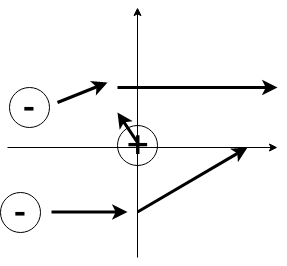
\includegraphics[width=0.8\linewidth]{fig40.png}
 \end{center}
 \caption{超電導メカニズム}
 \label{fig:40}
\end{figure}
%=============================================================
\newpage
\end{document}
